% Options for packages loaded elsewhere
\PassOptionsToPackage{unicode}{hyperref}
\PassOptionsToPackage{hyphens}{url}
%
\documentclass[
]{article}
\usepackage{amsmath,amssymb}
\usepackage{lmodern}
\usepackage{ifxetex,ifluatex}
\ifnum 0\ifxetex 1\fi\ifluatex 1\fi=0 % if pdftex
  \usepackage[T1]{fontenc}
  \usepackage[utf8]{inputenc}
  \usepackage{textcomp} % provide euro and other symbols
\else % if luatex or xetex
  \usepackage{unicode-math}
  \defaultfontfeatures{Scale=MatchLowercase}
  \defaultfontfeatures[\rmfamily]{Ligatures=TeX,Scale=1}
\fi
% Use upquote if available, for straight quotes in verbatim environments
\IfFileExists{upquote.sty}{\usepackage{upquote}}{}
\IfFileExists{microtype.sty}{% use microtype if available
  \usepackage[]{microtype}
  \UseMicrotypeSet[protrusion]{basicmath} % disable protrusion for tt fonts
}{}
\makeatletter
\@ifundefined{KOMAClassName}{% if non-KOMA class
  \IfFileExists{parskip.sty}{%
    \usepackage{parskip}
  }{% else
    \setlength{\parindent}{0pt}
    \setlength{\parskip}{6pt plus 2pt minus 1pt}}
}{% if KOMA class
  \KOMAoptions{parskip=half}}
\makeatother
\usepackage{xcolor}
\IfFileExists{xurl.sty}{\usepackage{xurl}}{} % add URL line breaks if available
\IfFileExists{bookmark.sty}{\usepackage{bookmark}}{\usepackage{hyperref}}
\hypersetup{
  pdftitle={Project 2 - Job Hunt},
  pdfauthor={Noah Love and Ido Li On},
  hidelinks,
  pdfcreator={LaTeX via pandoc}}
\urlstyle{same} % disable monospaced font for URLs
\usepackage[margin=1in]{geometry}
\usepackage{color}
\usepackage{fancyvrb}
\newcommand{\VerbBar}{|}
\newcommand{\VERB}{\Verb[commandchars=\\\{\}]}
\DefineVerbatimEnvironment{Highlighting}{Verbatim}{commandchars=\\\{\}}
% Add ',fontsize=\small' for more characters per line
\usepackage{framed}
\definecolor{shadecolor}{RGB}{248,248,248}
\newenvironment{Shaded}{\begin{snugshade}}{\end{snugshade}}
\newcommand{\AlertTok}[1]{\textcolor[rgb]{0.94,0.16,0.16}{#1}}
\newcommand{\AnnotationTok}[1]{\textcolor[rgb]{0.56,0.35,0.01}{\textbf{\textit{#1}}}}
\newcommand{\AttributeTok}[1]{\textcolor[rgb]{0.77,0.63,0.00}{#1}}
\newcommand{\BaseNTok}[1]{\textcolor[rgb]{0.00,0.00,0.81}{#1}}
\newcommand{\BuiltInTok}[1]{#1}
\newcommand{\CharTok}[1]{\textcolor[rgb]{0.31,0.60,0.02}{#1}}
\newcommand{\CommentTok}[1]{\textcolor[rgb]{0.56,0.35,0.01}{\textit{#1}}}
\newcommand{\CommentVarTok}[1]{\textcolor[rgb]{0.56,0.35,0.01}{\textbf{\textit{#1}}}}
\newcommand{\ConstantTok}[1]{\textcolor[rgb]{0.00,0.00,0.00}{#1}}
\newcommand{\ControlFlowTok}[1]{\textcolor[rgb]{0.13,0.29,0.53}{\textbf{#1}}}
\newcommand{\DataTypeTok}[1]{\textcolor[rgb]{0.13,0.29,0.53}{#1}}
\newcommand{\DecValTok}[1]{\textcolor[rgb]{0.00,0.00,0.81}{#1}}
\newcommand{\DocumentationTok}[1]{\textcolor[rgb]{0.56,0.35,0.01}{\textbf{\textit{#1}}}}
\newcommand{\ErrorTok}[1]{\textcolor[rgb]{0.64,0.00,0.00}{\textbf{#1}}}
\newcommand{\ExtensionTok}[1]{#1}
\newcommand{\FloatTok}[1]{\textcolor[rgb]{0.00,0.00,0.81}{#1}}
\newcommand{\FunctionTok}[1]{\textcolor[rgb]{0.00,0.00,0.00}{#1}}
\newcommand{\ImportTok}[1]{#1}
\newcommand{\InformationTok}[1]{\textcolor[rgb]{0.56,0.35,0.01}{\textbf{\textit{#1}}}}
\newcommand{\KeywordTok}[1]{\textcolor[rgb]{0.13,0.29,0.53}{\textbf{#1}}}
\newcommand{\NormalTok}[1]{#1}
\newcommand{\OperatorTok}[1]{\textcolor[rgb]{0.81,0.36,0.00}{\textbf{#1}}}
\newcommand{\OtherTok}[1]{\textcolor[rgb]{0.56,0.35,0.01}{#1}}
\newcommand{\PreprocessorTok}[1]{\textcolor[rgb]{0.56,0.35,0.01}{\textit{#1}}}
\newcommand{\RegionMarkerTok}[1]{#1}
\newcommand{\SpecialCharTok}[1]{\textcolor[rgb]{0.00,0.00,0.00}{#1}}
\newcommand{\SpecialStringTok}[1]{\textcolor[rgb]{0.31,0.60,0.02}{#1}}
\newcommand{\StringTok}[1]{\textcolor[rgb]{0.31,0.60,0.02}{#1}}
\newcommand{\VariableTok}[1]{\textcolor[rgb]{0.00,0.00,0.00}{#1}}
\newcommand{\VerbatimStringTok}[1]{\textcolor[rgb]{0.31,0.60,0.02}{#1}}
\newcommand{\WarningTok}[1]{\textcolor[rgb]{0.56,0.35,0.01}{\textbf{\textit{#1}}}}
\usepackage{graphicx}
\makeatletter
\def\maxwidth{\ifdim\Gin@nat@width>\linewidth\linewidth\else\Gin@nat@width\fi}
\def\maxheight{\ifdim\Gin@nat@height>\textheight\textheight\else\Gin@nat@height\fi}
\makeatother
% Scale images if necessary, so that they will not overflow the page
% margins by default, and it is still possible to overwrite the defaults
% using explicit options in \includegraphics[width, height, ...]{}
\setkeys{Gin}{width=\maxwidth,height=\maxheight,keepaspectratio}
% Set default figure placement to htbp
\makeatletter
\def\fps@figure{htbp}
\makeatother
\setlength{\emergencystretch}{3em} % prevent overfull lines
\providecommand{\tightlist}{%
  \setlength{\itemsep}{0pt}\setlength{\parskip}{0pt}}
\setcounter{secnumdepth}{-\maxdimen} % remove section numbering
\ifluatex
  \usepackage{selnolig}  % disable illegal ligatures
\fi

\title{Project 2 - Job Hunt}
\author{Noah Love and Ido Li On}
\date{3/4/2021}

\begin{document}
\maketitle

Code for the project can be found
\href{\%22https://github.com/noahlove/data-mining-project-2.git\%22}{here}

\hypertarget{introduction}{%
\subsection{Introduction}\label{introduction}}

The data provided to us for this report is a scraped job postings from
\href{https://www.indeed.com/}{indeed.com}. They were scraped from
September 2020 to March 2021, in four distinct scrapes.

The data is presented in a json file. It is a list of 16 - 25 (depending
on the scrape) lists, each representing a unique job category: i.e.~ux
designer, recruiter or marketing. Within each of the 16 lists, are 2
lists: the first is a list of 4, describing position, location, job time
(full or part time), and start time. The second list contains job
descriptions associated with that job category.

Here is an (shortened) example of how each job postings appears in JSON:

\begin{quote}
``2ccc2596d13c54d4'': ``Job to be done\nWe\u2019re the best way to get
better.\n\nAbout Buoy Health:\nBuoy builds a digital health tool that
helps people \u2013 from the moment they get sick \u2013 start their
health care on the right foot. Started by a team of doctors and computer
scientists working at the Harvard Innovation Laboratory in Boston MA,
Buoy was developed in direct response to the downward spiral we\u2019ve
all faced when we attempt to self-diagnose our symptoms online\ldots.''
\end{quote}

\hypertarget{clean-up-the-data}{%
\subsubsection{Clean up the data}\label{clean-up-the-data}}

Our first major choice was to combine all four data sets (different
dates) into one large csv. None of our questions necessarily related to
the time aspect of the data so we chose to just unify them. Here is an
example of the list of categories, and associated characteristics.

\begin{verbatim}
## # A tibble: 25 x 2
##    job_title               n
##    <chr>               <int>
##  1 actuary                61
##  2 business analyst      120
##  3 data architect        127
##  4 data journalist         5
##  5 data scientist        120
##  6 deep learning         114
##  7 econmist               71
##  8 engineering manager    82
##  9 financial analyst      79
## 10 financial engineer      6
## # ... with 15 more rows
\end{verbatim}

First, there are only 25 categories here. Definitely not a comprehensive
view of the job market, so if you are really set about going into a
field that is not listed, this loop project explained below would not be
a good fit. However, for most people majoring in statistics or computer
science, this might provide a nice survey of various jobs.

Another question that would be reasonable to ask is what is the
distribution of job postings per category?

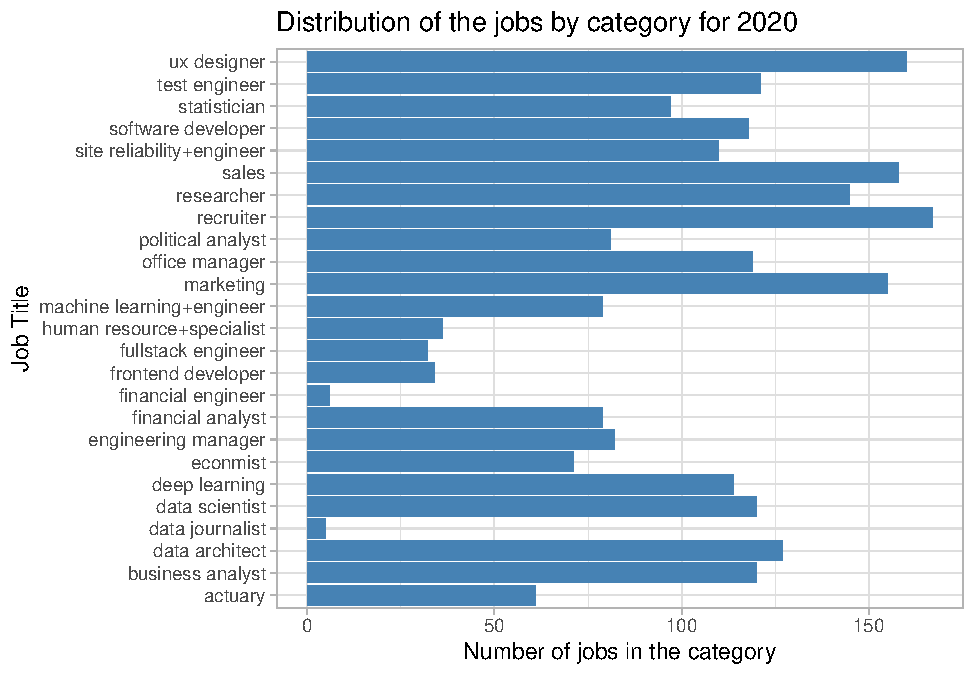
\includegraphics{main_files/figure-latex/unnamed-chunk-2-1.pdf}

Hopefully you don't want to be a data journalist because the data is not
as comprehensive than the rest. But otherwise, it seems to be very equal
across the categories. Otherwise, for the categories mentioned, it seems
that the data is representative and could be very useful in a job hunt
if you have interests in the related field.

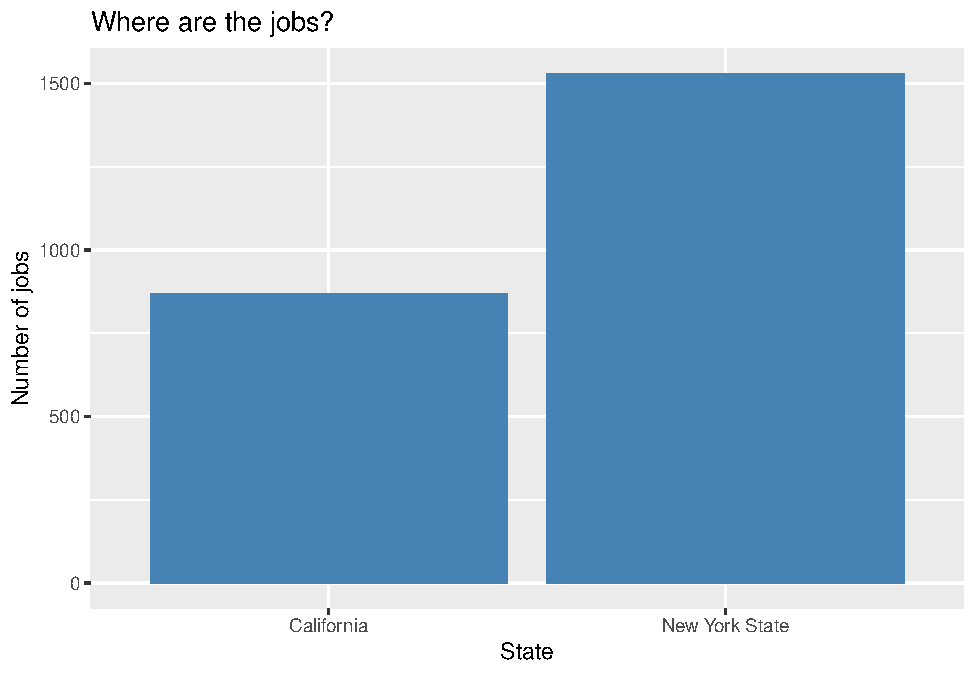
\includegraphics{main_files/figure-latex/unnamed-chunk-3-1.pdf} The data
is likely most lacking in location. For people that were hoping for
rural jobs, or maybe remote jobs, the data scraped is specifically
focused on California and New York State which is not for everyone.
Also, the data is particularly focused on mainly full time jobs. While
there are percentages of other types of jobs including contract,
internships and part-time, they are no where near as prevalent as full
time jobs.

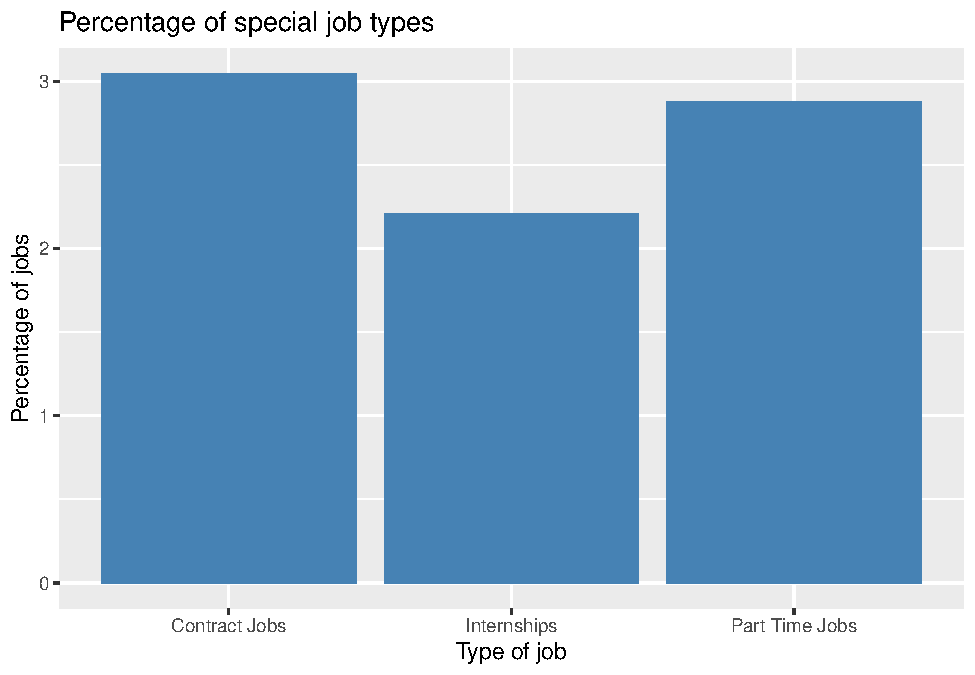
\includegraphics{main_files/figure-latex/unnamed-chunk-4-1.pdf}

\hypertarget{wrangle-the-data}{%
\subsection{Wrangle the data}\label{wrangle-the-data}}

We wrangled all of these into a csv format for easier working. The data
frame gives job location, salary minimum and maximum (rare), separate
columns for different types of job positions (full time, part time,
contract or internship) as well as job title (category), job\_id
(distinct id number from Indeed) and the job description from the
company.

\hypertarget{data-quality-issue}{%
\subsubsection{Data Quality Issue}\label{data-quality-issue}}

Some companies appear to have gotten lazy in their copy and pasting
between websites and have smashed some words together. Because it is a
rare enough occurrence, it will hopefully not have a large effect on the
data.

\hypertarget{data-processing}{%
\subsection{Data processing}\label{data-processing}}

The data was then tokenized using the package text2vec, as well as
broken into n-grams. Once the job descriptions were tokenized, then we
could proceed to create a cosine similarity matrix for the job postings,
identified by their Indeed ID. Cosine similiarity is a measure of
similarity between two vectors, in this case two job postings. The
values range from 0 to 1 (the same posting). This method was chosen
because of the type of data. Instead of having to come up with a clever
data normalization technique due to some companies being incredibly
verbose while others are super brief, this takes care of that instead.
Below is an example of the top left corner of the cosine matrix

\begin{verbatim}
## # A tibble: 4 x 4
##   X                e478b356032e70fd fa6dc34d522ab0d0 X844a7481ad8c3605
##   <chr>                       <dbl>            <dbl>             <dbl>
## 1 e478b356032e70fd            1.00             0.165             0.220
## 2 fa6dc34d522ab0d0            0.165            1                 0.180
## 3 844a7481ad8c3605            0.220            0.180             1    
## 4 51435069529900d2            0.219            0.154             0.216
\end{verbatim}

\hypertarget{user-input}{%
\subsection{User Input}\label{user-input}}

Now, we will ask for user input, in a somewhat manual way. Based on your
resume, we choose keywords from previous job positions, courses and
trainings that you think would be relevant to your job search.

How does this help? We will turn the words that are entered from your
resume into a unique tokenized string as well. This will be put into the
cosine similarity matrix, and we can compare which job postings you have
the most in common with. Using the post ID, we can then filter the job
postings such that you can get 3 recommendations from 3 distinct Indeed
job categories to give you a variety of options to choose from.

\begin{Shaded}
\begin{Highlighting}[]
\NormalTok{noah\_input }\OtherTok{\textless{}{-}} \StringTok{"Coins Gold Bullion Banking Diamonds Website Development Software Coding Programming Hedge Investment Fund Social Media Student Salesman Entrepreneurship, Startup, Incubator, HTML, R, Python"}

\NormalTok{ido\_input }\OtherTok{\textless{}{-}}  \StringTok{"Programming Cybersecurity Networks Reverse Engineering"}
\end{Highlighting}
\end{Shaded}

Here, Ido and Noah both provided key words from past education, job
descriptions and titles that were in our resume. For the sake of testing
both extremes, we have a more verbose input and a more concise one.

Here is a list of the most popular words use in job descriptions.

\begin{verbatim}
## Number of docs: 2399 
## 37 stopwords: a, an, and, are, as, at ... 
## ngram_min = 1; ngram_max = 3 
## Vocabulary: 
##          term term_count doc_count
## 1:       team       5457      1850
## 2:       will       6251      1910
## 3:       work       7001      2110
## 4:       data       7973      1395
## 5: experience       9195      2185
\end{verbatim}

Here is an example of the cosine similarity matrix. Noah's resume is the
same as itself so it has a similarity of 1. It is also interestingly
almost nothing like Ido's (very close to 0). In such a way, the two user
inputs actually serve as a great example of how different strings show
as very dissimilar and wouldn't be recommended. Ironically, we worked
great as partners so maybe our user input isn't completed representative
of us.

In this way, the similarity score provides a metric for how similar or
``good'' the match is to our resume and provided terms.

\begin{verbatim}
##                  RESUME (NOAH)
## RESUME (NOAH)     1.0000000000
## RESUME (IDO)      0.0029706255
## b8a95f829b9c6620  0.0006204078
## f4c84f7a3364f6f2  0.0013222891
## db27839785a0d533  0.0014726637
## db347273bff9c20a  0.0014201041
## fbf87e3c9ff3756b  0.0014726637
## 4f7e548e2296a623  0.0004667310
## 3f90f8de3315361b  0.0000000000
## 2db89e42fe22629e  0.0038598299
\end{verbatim}

As our way of creating diversity, we chose to separate by top posting
per job category. If you are using a service like entering keywords to
find a job, it is unlikely you know the exact field or even category of
job you want. So to ensure a diverse option, we first outputted the most
similar job posting to your resume in each job category. For example,
the first 10:

\begin{verbatim}
## # A tibble: 21 x 11
## # Groups:   job_title [21]
##    job_id           cos_simil job_location   is_fulltime is_parttime is_contract
##    <chr>                <dbl> <chr>          <lgl>       <lgl>       <lgl>      
##  1 01e29bad144f3aec   0.00387 New York State TRUE        FALSE       FALSE      
##  2 1329e487e7ec612c   0.00869 New York State TRUE        FALSE       FALSE      
##  3 179d177e73eb0d4f   0.0132  California     TRUE        FALSE       FALSE      
##  4 2239a60e34c8df76   0.0104  New York State TRUE        FALSE       FALSE      
##  5 22fc2bd09c7dbb62   0.00630 New York State TRUE        FALSE       FALSE      
##  6 2a046d74a41cad2e   0.00992 California     TRUE        FALSE       FALSE      
##  7 3f584e097c6c449b   0.00589 California     TRUE        FALSE       FALSE      
##  8 4f260377db0b3750   0.00869 New York State TRUE        FALSE       FALSE      
##  9 5879c9ef1c795e21   0.00738 New York State TRUE        FALSE       FALSE      
## 10 8898b3e31cf2342e   0.00874 New York State TRUE        FALSE       FALSE      
## # ... with 11 more rows, and 5 more variables: is_internship <lgl>,
## #   salary_min <int>, salary_max <int>, job_title <chr>, job_desc <chr>
\end{verbatim}

\hypertarget{data-issues-and-creating-additional-diversity}{%
\subsubsection{Data issues and creating additional
diversity}\label{data-issues-and-creating-additional-diversity}}

One of the largest issues with getting a diverse selection of jobs is
preventing the same company from being chosen multiple times. For
example, many companies even cross posted the exact same job into two
separate categories. Or they would post the exact same job, but have a
different ID because they were hoping to fill the job in California and
New York separately.

To fix these issues, we found there were two fixes. First, duplicate
entries, with the exact same (word-for-word) job description were
deleted. Second, we used n-grams to delete jobs from the same company.
We noticed that companies would post a brief description about the
company in the job description, so we could filter through them using
duplicate n-grams. If two job descriptions had 8 words in a row
duplicated with another job description, one of them was pruned from our
data. This prevented Ido for example from recieving 3 Palo Alto job
recommendations.

\hypertarget{ensuring-diverse-jobs}{%
\subsubsection{Ensuring diverse jobs}\label{ensuring-diverse-jobs}}

Our way of ensuring diverse jobs and provide interesting choices was to
use the job categories provided by indeed. Very few jobs were extremely
similar across categories, as there aren't a lot of similar words in a
marketing job as an actuary. So after finding the top job in each
category, we selected the top across those 25 categories. As a result,
we found that for various strings, there were often two somewhat similar
category jobs but then one much more diverse. As a result, it is likely
you miss out on some more fitted jobs in the name of a more diverse
selection but this makes job hunting a lot more fun.

However, just by choosing top by category doesn't mean we will be
similar to that category. In fact, even the ``best'' job for someone in
the category might still be really bad. For example, Noah's ``worst'' of
all the categories can be seen below, a full stack engineer (for Vox), a
position he is not well equipped for and decently far from his chosen
input.

\begin{Shaded}
\begin{Highlighting}[]
\NormalTok{bottom\_one}
\end{Highlighting}
\end{Shaded}

\begin{verbatim}
## # A tibble: 1 x 4
##   job_title      job_desc                                 job_location cos_simil
##   <chr>          <chr>                                    <chr>            <dbl>
## 1 fullstack eng~ "Full Job DescriptionAs the leading ind~ New York St~   0.00366
\end{verbatim}

However, the top three look very promising, good and diverse:

\begin{verbatim}
## # A tibble: 3 x 4
##   job_title    job_desc                                   job_location cos_simil
##   <chr>        <chr>                                      <chr>            <dbl>
## 1 statistician "Full Job DescriptionDescription\nJob Des~ California      0.0132
## 2 data scient~ "New York University: NYU - Domestic: Fac~ New York St~    0.0150
## 3 marketing    "Full Job DescriptionCompany Overview: Tr~ New York St~    0.0168
\end{verbatim}

As an example of a good match, here is one of my top results.

\begin{verbatim}
##                                                                                                                                                                                                                                                                                                                                                                                                                                                                                                             statistician 
## "Full Job DescriptionDescription\nJob Description:\nLeidos’s Military & Veterans Solutions Health Group is currently seeking a full-time Research Statistician to support the Warfighter Performance Department at the Naval Health Research Center in San Diego, CA. This position will provide direct support to the Sleep, Tactical Efficiency, and Endurance Laboratory (STEEL) and collaborating military commands and institutions. The candidate will help conduct research related to the US Navy’s Culture ..."
\end{verbatim}

\begin{verbatim}
## # A tibble: 3 x 3
##   job_title          job_desc                                      job_location 
##   <chr>              <chr>                                         <chr>        
## 1 office manager     "Reverse Mortgage Funding LLC is committed t~ New York Sta~
## 2 test engineer      "Full Job DescriptionField Test Engineers te~ New York Sta~
## 3 machine learning+~ "Full Job DescriptionCompany Description\nOu~ New York Sta~
\end{verbatim}

\hypertarget{measuring-diversity}{%
\subsubsection{Measuring Diversity}\label{measuring-diversity}}

To measure diversity, we decided to look at the similarity between our
final three choices. If these were high, we would know that they were
unlikely diverse. As such, we created a cosine similarly between the
final three choices and took the average up the upper corner to get a
``diversity score'' of our final selection. The closer to 0 would
represent more diverse, whereas closer to 1 means they are very similar.
For example, here is the similarity matrix for Ido's results as well as
his score.

\begin{verbatim}
##            1          2          3
## 1 1.00000000 0.01933331 0.02877068
## 2 0.01933331 1.00000000 0.02647846
## 3 0.02877068 0.02647846 1.00000000
\end{verbatim}

\begin{verbatim}
## Div. Score: 0.02486081
\end{verbatim}

\end{document}
